% Made up for the tikra benchmark.
% The first four periods of the periodic table, each element colored by its family.
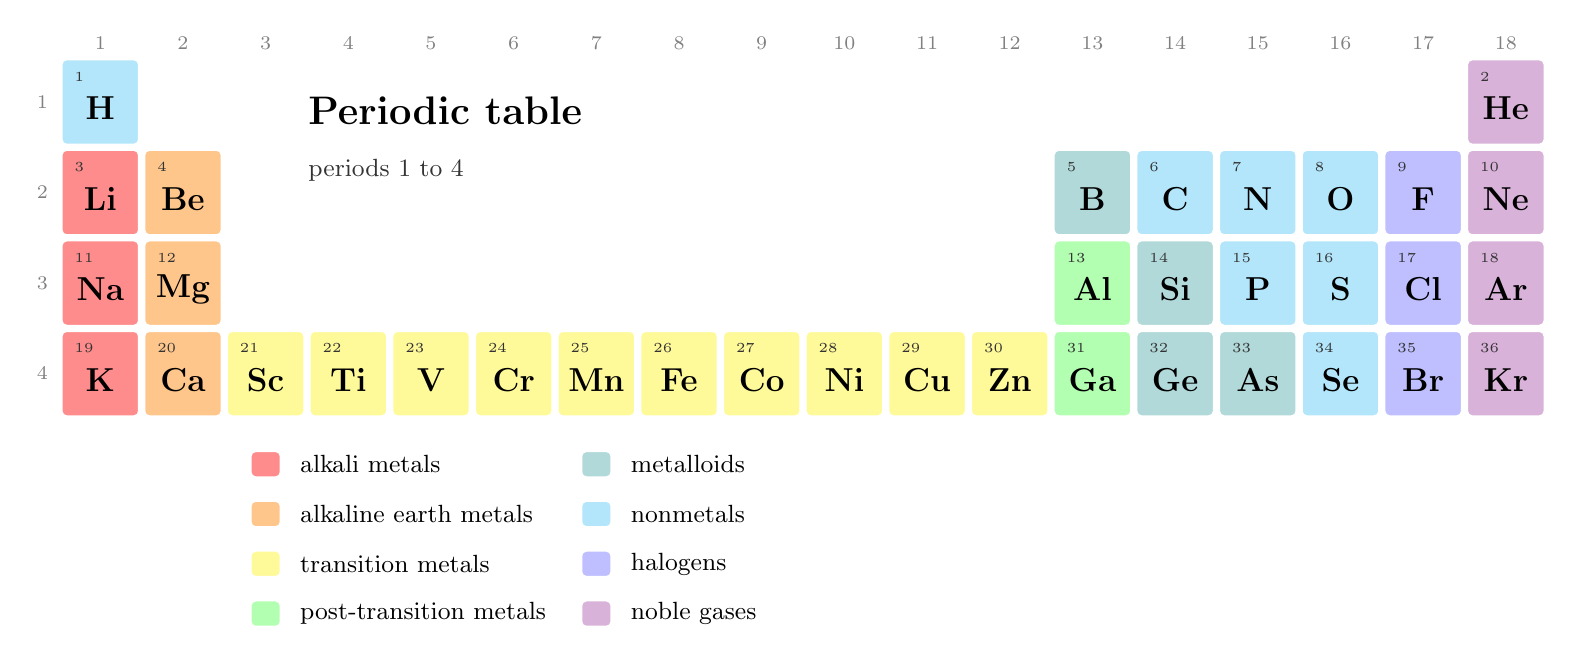
\begin{tikzpicture}[x=1.05cm, y=-1.15cm,
    cell/.style={draw=white, line width=1.2pt, rounded corners=2pt, minimum width=1.0cm, minimum height=1.1cm},
    alkali/.style={cell, fill=red!45}, alkaline/.style={cell, fill=orange!45},
    transition/.style={cell, fill=yellow!40}, post/.style={cell, fill=green!30},
    metalloid/.style={cell, fill=teal!30}, nonmetal/.style={cell, fill=cyan!30},
    halogen/.style={cell, fill=blue!25}, noble/.style={cell, fill=violet!30}]
  \foreach \s/\z/\g/\p/\f in {
      H/1/1/1/nonmetal, He/2/18/1/noble, Li/3/1/2/alkali, Be/4/2/2/alkaline,
      B/5/13/2/metalloid, C/6/14/2/nonmetal, N/7/15/2/nonmetal, O/8/16/2/nonmetal,
      F/9/17/2/halogen, Ne/10/18/2/noble, Na/11/1/3/alkali, Mg/12/2/3/alkaline,
      Al/13/13/3/post, Si/14/14/3/metalloid, P/15/15/3/nonmetal, S/16/16/3/nonmetal,
      Cl/17/17/3/halogen, Ar/18/18/3/noble, K/19/1/4/alkali, Ca/20/2/4/alkaline,
      Sc/21/3/4/transition, Ti/22/4/4/transition, V/23/5/4/transition, Cr/24/6/4/transition,
      Mn/25/7/4/transition, Fe/26/8/4/transition, Co/27/9/4/transition, Ni/28/10/4/transition,
      Cu/29/11/4/transition, Zn/30/12/4/transition, Ga/31/13/4/post, Ge/32/14/4/metalloid,
      As/33/15/4/metalloid, Se/34/16/4/nonmetal, Br/35/17/4/halogen, Kr/36/18/4/noble} {
    \node[\f] at (\g,\p) {};
    \node[font=\tiny, anchor=north west, gray!40!black] at ([xshift=-0.45cm, yshift=0.5cm]\g,\p) {\z};
    \node[font=\large\bfseries] at ([yshift=-0.08cm]\g,\p) {\s};
  }
  \foreach \g in {1,2,...,18} \node[font=\scriptsize, gray] at (\g,0.35) {\g};
  \foreach \p in {1,...,4} \node[font=\scriptsize, gray] at (0.3,\p) {\p};
  \node[font=\Large\bfseries, anchor=west] at (3.4,1.1) {Periodic table};
  \node[font=\small, anchor=west, gray!40!black] at (3.4,1.75) {periods 1 to 4};
  \foreach \f/\name [count=\i from 0] in {alkali/alkali metals, alkaline/alkaline earth metals,
      transition/transition metals, post/post-transition metals, metalloid/metalloids,
      nonmetal/nonmetals, halogen/halogens, noble/noble gases} {
    \pgfmathsetmacro\c{3 + 4*int(\i/4)}
    \pgfmathsetmacro\r{5 + 0.55*mod(\i,4)}
    \node[\f, minimum width=0.4cm, minimum height=0.35cm] at (\c,\r) {};
    \node[font=\small, anchor=west] at (\c+0.3,\r) {\name};
  }
\end{tikzpicture}
